\documentclass{article}
% basics
\usepackage{amsfonts}
\usepackage{enumitem}
\usepackage{float}
\usepackage{graphicx}
\usepackage{hyperref} 
\usepackage[labelfont=bf]{caption}

\newtheorem{theorem}{Theorem}
\newtheorem{lemma}[theorem]{Lemma}
\newtheorem{corollary}{Corollary}[theorem]

\usepackage{tikz}



% unique math expressions:  
\usepackage{amsmath}
\DeclareMathOperator*{\andloop}{\wedge}
\DeclareMathOperator*{\pr}{Pr}
\DeclareMathOperator*{\approach}{\longrightarrow}
\DeclareMathOperator*{\eq}{=}

% grey paper
\usepackage{xcolor}
% \pagecolor[rgb]{0.11,0.11,0.11}
% \color{white}

% embedded code sections
\usepackage{listings}
\definecolor{codegreen}{rgb}{0,0.6,0}
\definecolor{codegray}{rgb}{0.5,0.5,0.5}
\definecolor{codepurple}{rgb}{0.58,0,0.82}
\lstdefinestyle{mystyle}{
    commentstyle=\color{codegreen},
    keywordstyle=\color{magenta},
    numberstyle=\tiny\color{codegray},
    stringstyle=\color{codepurple},
    basicstyle=\ttfamily\footnotesize,
    breakatwhitespace=false,         
    breaklines=true,                 
    captionpos=b,                    
    keepspaces=true,                 
    numbers=left,                    
    numbersep=5pt,                  
    showspaces=false,                
    showstringspaces=false,
    showtabs=false,                  
    tabsize=2
}

\lstset{style=mystyle}

\begin{document}
\author{Yosef Goren, Andrew Elashkin}

\title{Introduction to Software Verification 236342, Homework 3}
\maketitle
\section*{Question 1}
\begin{enumerate}[label=\Alph*.]
    \item 3
    \item 1
    \item 3
    \item 2
    \item 4
    \item 1
    \item 4
    \item 3
    \item 2.
$\phi_1 \not\Rightarrow \phi_2$:
A counterexample of the kripke structure M and path $\pi$, that satisfies $\phi_1$, but not $\phi_2$ is below. Assume $\pi = s_0, s_0, s_0, ...$, then the pair $M, \pi \models \phi_1$, but $M, \pi \not\models \phi_2$.

\begin{center}
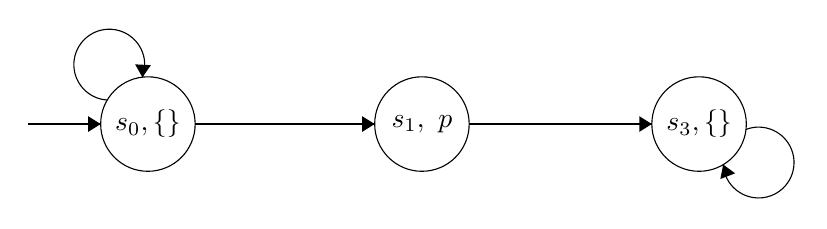
\begin{tikzpicture}[scale=0.2]
\tikzstyle{every node}+=[inner sep=0pt]
\draw [black] (18.9,-29) circle (3);
\draw (18.9,-29) node {$s_0,\mbox{\{\}}$};
\draw [black] (36.3,-29) circle (3);
\draw (36.3,-29) node {$s_1,\mbox{ }p$};
\draw [black] (53.9,-29) circle (3);
\draw (53.9,-29) node {$s_3,\mbox{\{\}}$};
\draw [black] (21.9,-29) -- (33.3,-29);
\fill [black] (33.3,-29) -- (32.5,-28.5) -- (32.5,-29.5);
\draw [black] (39.3,-29) -- (50.9,-29);
\fill [black] (50.9,-29) -- (50.1,-28.5) -- (50.1,-29.5);
\draw [black] (56.868,-29.345) arc (111.09476:-176.90524:2.25);
\fill [black] (55.43,-31.57) -- (55.25,-32.49) -- (56.19,-32.13);
\draw [black] (16.331,-27.474) arc (267.02387:-20.97613:2.25);
\fill [black] (18.55,-26.03) -- (19.09,-25.26) -- (18.09,-25.21);
\draw [black] (11.3,-29) -- (15.9,-29);
\fill [black] (15.9,-29) -- (15.1,-28.5) -- (15.1,-29.5);
\end{tikzpicture}
\end{center}

$\phi_2 \Rightarrow \phi_1$:
$$M, \pi \models EGFp \Rightarrow$$
$$ \forall i \geq 0, (M, \pi_i) \models Fp \Rightarrow$$
Since we know that the path $pi_i$ exists, we can say that for every node $s_i$ in the path $pi_i$ there is such a path:
$$ \forall i \geq 0, (M, s_i) \models EFp \Rightarrow$$
$$M, \pi \models EGEFp $$


    \item 1. 

$\phi_1 \Rightarrow \phi_2$:
$$ M,s \models AFAXp = A[true UAXp] \Rightarrow$$
For every path $\pi$ starting at s:
$$ \pi \models F A X p \Rightarrow \exists i \geq 0, \pi_i \models A X p \Rightarrow$$
$$\pi_i \models A F X p \Rightarrow \pi \models A F X p \Rightarrow $$
$$\pi \models X A F p \Rightarrow  M,s \models AXAFp$$


$\phi_2 \not\Rightarrow \phi_1$: A counterexample of the kripke structure M and path $\pi$, that satisfies $\phi_2$, but not $\phi_1$ is below. Assume $\pi = s_0, s_1, s_0, s_1, ...$, then the pair $M, \pi \models \phi_2$, but $M, \pi \not\models \phi_1$.

\begin{center}
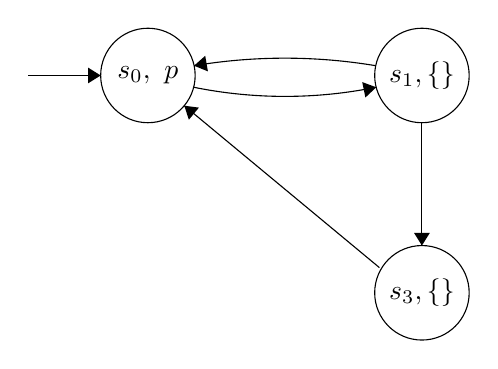
\begin{tikzpicture}[scale=0.2]
\tikzstyle{every node}+=[inner sep=0pt]
\draw [black] (18.9,-29) circle (3);
\draw (18.9,-29) node {$s_0,\mbox{ }p$};
\draw [black] (36.3,-29) circle (3);
\draw (36.3,-29) node {$s_1,\mbox{\{\}}$};
\draw [black] (36.3,-42.8) circle (3);
\draw (36.3,-42.8) node {$s_3,\mbox{\{\}}$};
\draw [black] (33.396,-29.747) arc (-78.52785:-101.47215:29.141);
\fill [black] (33.4,-29.75) -- (32.51,-29.42) -- (32.71,-30.4);
\draw [black] (36.3,-32) -- (36.3,-39.8);
\fill [black] (36.3,-39.8) -- (36.8,-39) -- (35.8,-39);
\draw [black] (11.3,-29) -- (15.9,-29);
\fill [black] (15.9,-29) -- (15.1,-28.5) -- (15.1,-29.5);
\draw [black] (33.6,-41.2) -- (21.21,-30.92);
\fill [black] (21.21,-30.92) -- (21.5,-31.81) -- (22.14,-31.04);
\draw [black] (21.834,-28.379) arc (99.4996:80.5004:34.937);
\fill [black] (21.83,-28.38) -- (22.71,-28.74) -- (22.54,-27.75);
\end{tikzpicture}
\end{center}
\end{enumerate}

\section*{Question 2}

\begin{enumerate}
    \item Correct.
    \item Wrong.
    \item Wrong.
    \item Wrong.
    \item 4
    \item Wrong.

\end{enumerate}

\section*{Question 2}
\begin{enumerate}
    \item True. Let $\pi=s_0\rightarrow s_5\rightarrow s_5$.
        \begin{itemize}
            \item $M,\pi^2\models b$
            \item $M,\pi^1\models Xb$
            \item $M,\pi^0\models XXb$
            \item $M\models E[XXb]$
        \end{itemize}
    \item True. Let $\pi$ be an arbitrary path in $M$.\\
        $\pi$ must be in the form $s_0\rightarrow v\rightarrow *$
        where $v\in\{s_1,s_4,s_5\}$.\\
        We want to prove $M,\pi\models (EXa)U(EXc)$.\\
        \[\left((s_0,s_1)\in M\right)\wedge\left(s_1\models a\right)\Rightarrow s_0\models EXa\Rightarrow \pi^0\models EXa\]
        Additionally:
        \[\forall u\in\{s_1,s_4,s_5\}, \exists u':(u,u')\in M\wedge u'\models c\]
        \[\Rightarrow \forall u\in\{s_1,s_4,s_5\}, u\models EXc\]
        \[\Rightarrow v\models EXc\Rightarrow \pi^1\models EXc\]
        \[\Rightarrow M,\pi\models (EXa)U(EXc)\]
    \item True. Let $\pi=s_0\rightarrow s_4\rightarrow s_7$.
        \begin{itemize}
            \item $M,\pi^2\models Gc$
            \item $M,\pi^1\models a$
            \item $M,\pi^1\models aU(Gc)$
            \item $M,\pi^0\models b$
            \item $M,\pi^0\models bU(U(Gc))$
            \item $M\models E[bU(U(Gc))]$
        \end{itemize}
    \item True. Let $\pi=s_0\rightarrow *$.\\
        \begin{itemize}
            \item $s_0\models b$
            \item $s_0\models cUb$
            \item $s_0\models aU(cUb)$
            \item $\pi\models aU(cUb)$
        \end{itemize}
        $\Rightarrow M\models A[aU(cUb)]$
    \item False. Let $\pi=s_0\rightarrow s_1 \rightarrow s_2 \rightarrow s_3 \rightarrow s_3 \rightarrow ... $ \\ On this path $s_2 \models c$, meaning that $(Xa \rightarrow GXb)$ also needs to be satisfied for the formula to hold. $s_2 \models Xa$, but $s_3 \not\models GXb$ and so the formula does not hold for any path.
    \item False. $\phi_1 = FG(a \vee c)$ has to hold for any path from $s_0$. Let $\pi=s_0\rightarrow s_5 \rightarrow s_5 \rightarrow ... $ \\ $FG(a \vee c)$ does not hold for this path and so $M \not\models \phi$.
\end{enumerate}



\section*{Question 3}
\subsection*{Part A.}
Let: $H:=\{f_1\times f_2\times, ...,\times f_m\}$.\\
In other words, $H$ is the set of all possible combinations of the $m$ functions in $F$.\\
For any $h\in H, i\in[m]$, let $h[i]$ be an item within $h$
which was chosen from $f_i$ - one must exists since $h$ is a combination of $f_i$.\\
More formally, let $h[i]:= argmin_{i\mid s_i\in h\cap f_i}$ (the minimal item in $h$ from $f_i$).\\

Proof.\\
The following logical formulas are equivalent (and the transition from one to the other is trivial):
\begin{enumerate}
    \item $\forall i\in[m], f_i\cap inf(\pi)\neq\emptyset$
    \item $\forall i\in[m],\exists s_i, s_i\in f_i\wedge s_i\in inf(\pi)$
    \item $\forall i\in[m],\exists s_i\in f_i, s_i\in inf(\pi)$
    \item $\exists s_1,s_2,...,s_m,\forall i\in[m], s_i\in f_i\wedge s_i\in inf(\pi)$
    \item $\exists h\in H,\forall i\in[m], h[i]\in f_i\wedge h[i]\in inf(\pi)$
    \item $\exists h\in H,(\forall i\in[m], h[i]\in f_i)\wedge (\forall i\in[m], h[i]\in inf(\pi))$
    \item $\exists h\in H,(h\subseteq inf(\pi))\wedge (\forall i\in[m], h[i]\in inf(\pi))$
    \item $\exists h\in H,(h\subseteq inf(\pi))\wedge (true)$
    \item $\exists h\in H, h\subseteq inf(\pi)$
\end{enumerate}

\subsection*{Part B.}
For any $i\in[m], \bar{f_i}:=S\setminus f_i$.\\
Let $h:=\bigcap_{i=1}^m\bar{f_i}, H:=\{h\}$.\\

Proof.\\
The following series of formulas are equivalent:
\begin{enumerate}
    \item $\forall i\in[m], f_i\cap inf(\pi)=\emptyset$
    \item $\forall i\in[m], \bar{f_i}\cap inf(\pi)=inf(\pi)$
    \item $\forall i\in[m], inf(\pi)\subseteq \bar{f_i}$
    \item $\forall i\in[m], \forall s\in inf(\pi),s\in\bar{f_i}$
    \item $\forall s\in inf(\pi), \forall i\in[m],s\in\bar{f_i}$
    \item $\forall s\in inf(\pi), s\in\bigcap_{i=1}^m\bar{f_i}$
    \item $inf(\pi)\subseteq bigcap_{i=1}^m\bar{f_i}$
    \item $inf(\pi)\subseteq h$
    \item $\forall h'\in H, inf(\pi)\subseteq h'$
\end{enumerate}

\section*{Question 4}
\subsection*{Part A.}
Let $\phi_{B\rightarrow W}:=b\wedge E(bU(EGw))$,\\
Let $\phi_{W\rightarrow B}:=w\wedge E(wU(EGb))$.\\
The meaning of $\phi_{B\rightarrow W}$ is that there exists 
a path that starts with at-least one $b$, and then continues
being $b$ right untill the point where there exists a path satisfying $Gw$, meaning it
is $w$ exclusively from forever. In other words - 
by concatenating the 'inner' path that satisfies $Gw$ with the suffix of
the path that satisfies $\phi_{B\rightarrow W}$, we get a path
that has exactly one transision from $b$ to $w$ and no
transisions from $w$ to $b$.\\
Symmetrically, $\phi_{W\rightarrow B}$ means there exists a path
from the initial node that has
exactly one transision from $w$ to $b$ and no other transisions.\\
So $\phi_{W\rightarrow B}\vee \phi_{B\rightarrow W}$ is a 
satisfactory and required for the existance of a legal path.\\
Let $\phi:=\phi_{W\rightarrow B}\wedge \phi_{B\rightarrow W}$.\\
So $M,s\models \phi$ means that there exists a legal path from $s$.\\
To describe $\phi$ explicitly: 
\[
    \phi=
    (b\wedge E(bU(EGw)))\vee
    (w\wedge E(wU(EGb)))
\]

\subsection*{Part B.}
Define an algorithm for verifying $\phi$ as follows:
\begin{enumerate}
    \item Create $M':=(S,R',L)$, where $R':=\{(s,s')\in R\mid l(s)=l(s')\}$
        meaning nodes are now connected if they have the same color.
    \item Find the maximaly connected componenets of $M'$ - each componenet has uniform color.
    \item Mark with $C$ all components that have a circle, and recursively mark
    it with $C$ all nodes that have a path to a component with $C$.
    \item Now each component that has an inifinite path of just one color is marked
    with $C$. Moreover, each node that has an inifinite path of uniform color is within
    a component that is marked with $C$.
    \item Mark all black components that have $C$ with $E(wU(EGb))$ - note how
    all nodes within such a component actually satisfy this formula in the origina kripke structure.\\
    \item Symmetrically, mark all white components that have $C$ with $E(bU(EGw))$.
    \item Look at all edges (in the original structure) that go from 
    componenets of different colors. If there exists such edge between a
    white component and a $E(wU(EGb))$ component, mark the white component with $w\wedge E(wU(EGb))$,
    moreover, mark all white components leading to said white component also with $w\wedge E(wU(EGb))$.\\
    Note how each node within these white components indeed satisfy $w\wedge E(wU(EGb))$ in the
    original structure.\\
    Symmetrically, if there exists an edge between a black component and a $E(bU(EGw))$ component,
    mark the black component with $b\wedge E(bU(EGw))$ and all black components leading to said
    black component with $b\wedge E(bU(EGw))$ also.\\
    \item Now any node is legal iff it is marked with either $w\wedge E(wU(EGb))$ or $b\wedge E(bU(EGw))$,
    since if it was a legal node it either had to go from white to black or black to white - 
    which in either case would mean it is marked with either $w\wedge E(wU(EGb))$ or $b\wedge E(bU(EGw))$ respectively.
\end{enumerate}



\end{document}
